\documentclass[10pt]{article}
\usepackage[margin=.7in]{geometry}
\usepackage{amsthm}
\usepackage{hyperref}
\usepackage{graphicx}
\usepackage{booktabs}
\listfiles

\begin{document}
 
\begin{center}
\large
\hfill Okeefe Niemann\\
\hfill 4/28/2014\\
\hfill 1281465\\
\hfill PHYS 115 \\
\LARGE \textbf{Assignment 4}\\
\end{center}
\normalsize
%%%%%%%%%%%%%%%%%%%%%%%%%%%%%%%%%%%%%%%%%%%%%%%%%%%%%%%%%%%%%%%%%%%%%%%%%%%%%%%%%%%%%%%%%%%%%%%%%%%%%%%%%%
\section*{Question 2}
\subsection*{Part a: R2K}
\begin{itemize}
\item Input:
\begin{verbatim}
//Functions derivs and rk2 omitted, both were taken from Assignment 3 (question 6)

main()
{
 
        int M = 2; 
// specify the no. of variables
 
        double x[M], h, T, t, n, total_time, en, exact; 
// x is an array of size M
 
        void derivs(); 
// derivs computes the derivatives
 
        int i, j;

// maximum amplitudes which will be applied to rk2

        printf("\nTime    Energy    Deviation\n");

        x[0] = 1;
        x[1] = 0; //initializes p = 0
        T = 7.416; //Taken from assignment 3, question 6
        h = 0.02 * T; //defines the time steps
        n = T / h; //number of steps
        int period[3] = {1, 10, 100}; //periods run over
        exact = 0.25; //analytic value of energy

        for (i = 0; i < 3; i++)
        {
                n = period[i] * T / h;
                printf("Number of periods: %d\n", period[i]);
                t = 0;
                
                for(j = 0; j < n; j++)
                {
                        if(en < 2e31 -1)  //kills the loop if value is greater than double capacity
                        { 
                        rk2(t, x, derivs, h, M);
                        en = .5*x[1]*x[1] + .25*pow(x[0], 4);
                        t += h;
                        printf("%.5f   %.5f   %.5e\n",  t, en, (en-exact));
                        }
                        else
                                break;
               }
       }

return 0;
}
\end{verbatim}
\item: Output
\begin{verbatim}
Time        Energy    Deviation
Number of periods: 1
  ...        ...        ...
7.41600   2.52677e-01   2.67668e-03

Number of periods: 10
  ...        ...        ...
74.16000   0.28444   3.44409e-02

Number of periods: 100
  ...        ...          ...
633.77136   1.79083e+18   1.79083e+18
\end{verbatim}

\textbf{Comment:} When computing 100 periods, the deviation blows up and exceeds the capacity of the double number type. The above amount refers to the last returned number. 

\subsection*{Part b: Leapfrog}
\item Input:
\begin{verbatim}
#include<stdio.h>
#include<math.h>

double f(double x)
{
        return -pow(x, 3);
}

int main()
{
        int i, j, n;
        double x, p, T, t, h, exact, en, f();
        printf("\nTime    Energy    Deviation\n");
        
        x = 1; // initializes x
        p = 0; //initializes p
        T = 7.416;                      //Taken from assignment 3, question 6
        h = 0.02 * T;                   //defines the time steps
        int period[3] = {1, 10, 100};   //how many periods which will be run
        exact = 0.25;                   //exact value of the energy

        for (i = 0; i < 3; i++)
        {
                n = period[i] * T / h;

                printf("Number of periods: %d\n", period[i]);
                
                t = 0;
                
                for(j = 0; j < n; j++)
                {
                        if(en < pow(2,31) -1)
                        { 
                                x += .5 * h * v;
                                v += h * f(x);      //leapfrog method
                                x += .5 * h * v;
                                
                                en = .5 * pow(v, 2) + .25 * pow(x, 4);  //energy
                                t += h;	                               //adds time step
                                printf("%.5f   %.5e   %.5e\n",  t, en, (en-exact));
                        }
                        else
                                break;
                 }
        }

return 0;
}
\end{verbatim}
\item Output:

\begin{verbatim}
Time       Energy        Deviation
Number of periods: 1
  ...        ...           ...
7.41600   2.50004e-01   4.41068e-06

Number of periods: 10
  ...         ...           ...
74.01168   2.50088e-01   8.75189e-05

Number of periods: 100
  ...           ...           ...
741.60000   2.52046e-01   2.04589e-03

\end{verbatim}
\textbf{Comment:} As opposed to the Runge-Kutta 2 technique, the leapfrog method is much more precise and can hold a consisten value for larger numbers of periods. This is due to the fact that the leapfrog algorithm is symplectic, while RK2 does not preserve area as efficiently. 

%%%%%%%%%%%%%%%%%%%%%%%%%%%%%%%%%%%%%%%%%%%%%%%%%%%%%%%%%%%%%%%%%%%%%%%%%%%%%%%%%%%%%%%%%%%%%%%%%%%%%%%%%%%%
\section*{Question 3}
\subsection*{Part a}
See handwritten page for analytic solution.

\subsection*{Part b: Circular Orbit}
\item Input:
\begin{verbatim}
int main()
{
        int i, j;
        double en, r, t, period, h, n, x, y, p_x, p_y, f(), g(), leapfrogy(), leapfrogx();
        FILE* fout;
        
        fout = fopen("wienerslol.txt", "w");  //exports output to .txt
        x = 1;
        y = 0; 
        p_x = 0;                             //initial conditions
        p_y = 1;
        h = 0.0002 * period;                          //time step
        period = 2 * M_PI;
        n = period / h;                      //number of time steps
        
        fprintf(fout,"t              x         y          r       theta         en\n");
        
        for (i = 0; i < n; i++)
        {
                x += .5 * h * v_x;             //leapfrog for both x and y components
                y += .5 * h * v_y;
                p_x += h * f(x, y);
                p_y += h * g(x, y);
                x += .5 * h * v_x;
                y += .5 * h * v_y;
                
                r = pow(x*x  + y*y, 0.5);      //changes coordinates to r
                en = .5 * (p_x*p_x + p_y*p_y) + 1 / r;           //energy
                t += h;
                fprintf(fout,"%f   %f   %f   %f  %f   %f\n", t, x, y, r, atan2(y, x), en);
        }
        fclose(fout);
}
\end{verbatim}
\item Output:
\begin{center}
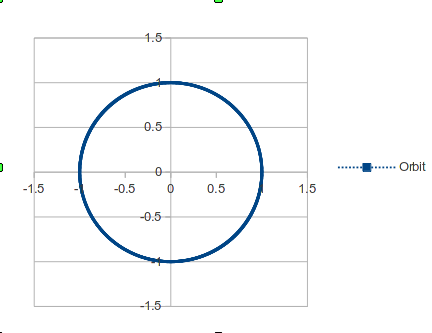
\includegraphics[scale=.7]{CircularOrbit}
\end{center}
\begin{verbatim}
t              x         y          r       theta      energy
0.010000   1.000000   0.010000   1.000050  0.009999   1.499975
0.020000   0.999900   0.019999   1.000100  0.019998   1.499950
 ...          ...       ...        ...       ...         ...
2.160000   -0.551510   0.831428   0.997716  2.156485   1.501147
2.170000   -0.559824   0.825830   0.997697  2.166531   1.501157
 ...          ...       ...        ...       ...         ...
4.470000   -0.245048   -0.970741   1.001192  -1.818064   1.499405
4.480000   -0.235341   -0.973094   1.001148  -1.808088   1.499427
 ...          ...       ...        ...       ...         ...
6.270000   0.999843   -0.013394   0.999933  -0.013396   1.500033
6.280000   0.999977   -0.003395   0.999983  -0.003395   1.500008
\end{verbatim}

\subsection*{Part c: Elliptical Orbit}
\item Input: \\
\textbf{Comment:} The input was the same as the above, but with a different initial momentum ($p_y = 0.7$) and the inclusion of the z-component of the angular momentum ($L_z = xp_y - yp_x$).

\item Output:
\begin{center}
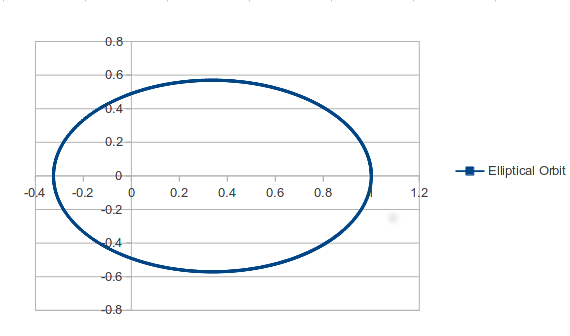
\includegraphics[scale=.5]{EllipticalOrbit}

\footnotesize Elliptical orbit with n = 500 timesteps.
\end{center}
\begin{verbatim}
   t          x         y          r       theta       energy   ang. momentum 
0.006772   0.999977   0.004741   0.999988  0.004741   -0.755000    0.700000
0.013545   0.999908   0.009481   0.999953  0.009482   -0.755000    0.700000
  ...        ...        ...        ...       ...         ...        ...
1.374817   -0.004854   0.487500   0.487524  1.580753   -0.755048    0.700000
1.381590   -0.014527   0.482372   0.482591  1.600902   -0.755050    0.700000
  ...        ...        ...        ...       ...         ...        ...
2.018204   0.004571   -0.492474   0.492495  -1.561514   -0.755047    0.700000
2.024977   0.014241   -0.497224   0.497428  -1.542163   -0.755045    0.700000
  ...        ...        ...        ...       ...         ...        ...
3.379477   0.999974   -0.005357   0.999988  -0.005357   -0.755000    0.700000
3.386249   1.000000   -0.000617   1.000000  -0.000617   -0.755000    0.700000
\end{verbatim}
\textbf{Comment:} As seen above, the energy of the system oscillates slightly due to rounding errors, though the angular momentum remains constant throughout the elliptical orbit to machine precision.

\subsection*{Part d: Timestep Comparison}
\item Input:\\
The input was taken from parts $b$ and $c$, with the timesteps $n=50$. 

\item Output: \\
\textbf{Circular Orbit:}
\begin{verbatim}
   t           x         y          r        theta        en
0.125664   0.992151   0.125171   1.000015   0.125498   1.499969
0.251327   0.968727   0.248376   1.000062   0.250988   1.499877
  ...         ...       ...        ...       ...         ...
3.392920   -0.976801  -0.231514  1.003862  -2.908874   1.492314
3.518584   -0.940405  -0.351037  1.003787  -2.784328   1.492462
  ...         ...       ...        ...        ...        ...
6.157522   0.987524   -0.157578  1.000018  -0.158234   1.499965
6.283185   0.999464   -0.032731  1.000000  -0.032737   1.500000
\end{verbatim}
\textbf{Elliptical Orbit:}
\begin{center}
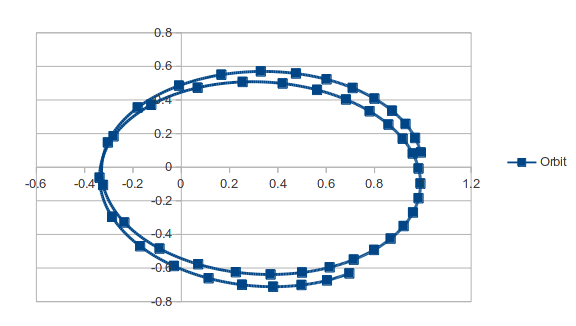
\includegraphics[scale=.5]{EllipticalOrbit1}

\footnotesize Elliptical orbit with n = 50 timesteps. More than one period displayed to show deviation from orbit.
\end{center}
\textbf{Comment:} As seen above, the radius of the circular orbit is relatively consistent after a full period, whereas the elliptical orbit steadily loses accuracy with a lower step size count.

\subsection*{Part e}
\textbf{Comment:} Analytic solution is located on the handwritten page in the back of this assignment.

\textbf{Numerical Results:}
\begin{verbatim}
t          ang. momentum 
0.012566   0.7000000000000001
0.025133   0.7000000000000000
  ...            ...
2.701770   0.7000000000000003
2.714336   0.7000000000000004
  ...            ...
3.379477   0.7000000000000003
3.386249   0.7000000000000004
\end{verbatim}
The above data was taken from part c, focusing on angular momentum with significant figures equal to machine precision for type double.

%%%%%%%%%%%%%%%%%%%%%%%%%%%%%%%%%%%%%%%%%%%%%%%%%%%%%%%%%%%%%%%%%%%%%%%%%%%%%%%%%%%%%%%%%%%%%%%%%%
\section*{Question 4}
\subsection*{Part a}
\textbf{Comment:} See back handwritten page for analytic solution.

\subsection*{Part b}
\item Input:
\begin{verbatim}
#include<stdio.h>
#include<math.h>

double f(double p)    //1st order derivative function
{
        return p;
}

double g(double x)    //2nd order derivative function
{
        return -1 * M_PI * M_PI * x;
}

int main()
{
        double h, x, x0, x1, x2, p0, p1, p2, f(), g(), k1x, k2x, k3x, k4x, k1p, k2p, k3p, k4p;
        int i, j, n, a, b;
        double hvalue[3] = {.2, .1, .05};
        
        printf("   x            f(x)           f'(x)\n");
        
        for(j = 0; j < 3; j++)
        {
                x = 0;
                a = 0;
                b = 1;
                x0 = 0;
                p0 = 1.0;			//Sets initial values
                h = hvalue[j];
                n = b / h;
                x2 = x0;
                p2 = p0;
                
                printf("h = %.2f\n", hvalue[j]);
                printf("%f      %f      %f\n", x, x2, p2);
                
                for (i = 0; i < n; i++)
                {
                        x1 = x2;
                        p1 = p2;
                        k1x = f(p1);
                        k1p = g(x1);
                        k2x = f(p1 + h / 2.0 * k1p);
                        k2p = g(x1 + h / 2.0 * k1x);
                        k3x = f(p1 + h / 2.0 * k2p);    //Runga Kutta 4 Method
                        k3p = g(x1 + h / 2.0 * k2x);
                        k4x = f(p1 + h * k3p);
                        k4p = g(x1 + h * k3x);
                        x2 = x1 + h / 6.0 * (k1x + 2.0*k2x + 2.0*k3x + k4x); 
                        p2 = p1 + h / 6.0 * (k1p + 2.0*k2p + 2.0*k3p + k4p);
                        x += h;
                }
                printf("%f      %f     %f\n", x, x2, p2);
        }

return 0;
}
\end{verbatim}
\item Output:
\begin{verbatim}
   x            f(x)         f'(x)
h = 0.20:
0.000000      0.000000      1.000000
1.000000      0.001118     -0.997964
h = 0.10:
0.000000      0.000000      1.000000
1.000000      0.000078     -0.999934
h = 0.05:
0.000000      0.000000      1.000000
1.000000      0.000005     -0.999998
\end{verbatim}
%%%%%%%%%%%%%%%%%%%%%%%%%%%%%%%%%%%%%%%%%%%%%%%%%%%%%%%%%%%%%%%%%%%%%%%%%%%%%%%%%%%%%%%%%%%%%%%%%%%%%%%%
\section*{Question 5}
\subsection*{Part i/ii/iii}
\item Input:
\begin{verbatim}
#include <stdio.h>
#include <time.h>
#include <stdlib.h>

int N = 1000;

main()
{
        int k, i, j, mid, x_l, x_h;
        double x[N], y, temp, f();
        
        //Generates N random numbers
        for(k = 0; k < N; k++) 
                x[k] = rand() / (RAND_MAX + 1.0);
   
        //Sorts random numbers in order from least to greatest
        for(i = 0; i < N - 1; i++)
        {
                for(j = 0; j < (N - 1 - i); j++)
                {
                        if(x[j] > x[j + 1])
                        {
                                temp = x[j];
                                x[j] = x[j+1];
                                x[j + 1] = temp;
                        }
                        else
                                continue;
                }
        }
        
        printf("Sorted Numbers:\n");

        for (i =0; i < 5; i++)
                printf("%f\n", x[i]);

        printf("  ...  \n");
        
        for(i = N-5; i < N; i++)
                printf("%f\n", x[i]);

        printf("\n");

        x_l = 0;
        x_h = N-1;

        //Uses the bisection method until element numbers of the array differ by one around 0.7
        while(x_h - x_l > 1)
        {
                mid = (x_h + x_l) / 2;

                if (x[mid] < 0.7)
                        x_l = mid + 1;

                else if(x[mid] > 0.7)
                        x_h = mid - 1;
        }

          /*+= 1 in printf statements take into account that the above while statement runs 
            one more time than needed before terminating*/
          printf("Closest number below 0.7:  %f \n", x[x_l - 1]); 
          printf("Closest number above 0.7:  %f \n", x[x_h + 1]);	

return 0;
}
\end{verbatim}
\item Output:
\begin{verbatim}
Sorted Numbers:
0.001125
0.002828
0.003231
0.003579
0.004162
  ...  
0.995300
0.997799
0.997970
0.998925
0.999994

Closest number below 0.7:  0.699075 
Closest number above 0.7:  0.700301 
\end{verbatim}


\subsection*{Part iv}
\item Input:
\begin{verbatim}
clock_t start = clock();
(sorting function, ran twice for N=10000 and N=20000)
clock_t end = clock();
double elapsed_time = (end-start)/(double)CLOCKS_PER_SEC;
printf("%f\n", elapsed_time);
\end{verbatim}
\item Output:
\begin{verbatim}
0.490000
1.870000
\end{verbatim}

\textbf{Comment:} As can be seen from the output, increasing the amount of numbers to be sorted increased the process time by about a factor of four. 

%%%%%%%%%%%%%%%%%%%%%%%%%%%%%%%%%%%%%%%%%%%%%%%%%%%%%%%%%%%%%%%%%%%%%%%%%%%%%%%%%%%%%%%%%%%%%%%%%%%%%%%%%%%%
\section*{Question 6}
\item: Input:
\begin{verbatim}
#include <stdio.h>
#include <math.h>


int  i, j, k, N, xdata, x[200];
double ydata, yerrordata, y[200], yerror[200], U[2][2], v[2], U_inv[2][2], Delta, a[2], 
       sigma[2], f[200], chi_squared;

FILE* fout;

int main()
{
        fout = fopen("statsdata.txt", "r");
        
        //Imports data
        while(fscanf(fout, "%d %lf %lf", &xdata, &ydata, &yerrordata) != EOF)
        {
                x[i] = xdata;
                y[i] = ydata;
                yerror[i++] = yerrordata;
        }

        N = 200;
        
        //Calulates symmetric 2x2 Matrix from x values
        for(i = 0; i < 2; i++)
        {
                for(j = 0; j < 2; j++)
                {
                        for(k = 0; k < 200; k++)
                                 U[i][j] += pow(x[k], i+j);
                }

        }
        
        //Calculates value needed to find parameters
        for(i = 0; i < 2; i++)
        {
                for(j = 0; j < N; j++)
                {
                         v[i] += y[j] * pow(x[j], i);
                }
        }

        //Determinant of above 2x2 matrix
        Delta = U[0][0]*U[1][1] - U[0][1] * U[0][1];
        
        //Creates inverse of the above 2x2 matrix
        U_inv[0][0] = U[1][1] / Delta;
        U_inv[0][1] = -U[0][1] / Delta;
        U_inv[1][0] = -U[0][1] / Delta;
        U_inv[1][1] = U[0][0] / Delta;
        
        //Calculates the two parameters from above inverted matrix and constant
        for(i = 0;  i < 2; i++)
        {
                for(j = 0; j < 2; j++)
                {
                        a[i] += U_inv[i][j] * v[j];
                }
        }
        
        //Calculates the error of the parameters
        for(i = 0; i < 2; i++)
        {
                sigma[i] = sqrt(U_inv[i][i]);
        }
        
        printf("a = %f p/m %f  (slope)\n", a[0], sigma[0]);
        printf("b = %f p/m %f  (y-intercept)\n", a[1], sigma[1]);
        
        //Calculates the chi-squared value per degree of freedom
        for(i = 0; i < N; i++)
        {
                f[i] = a[0] + a[1]*x[i];
                chi_squared += pow(((y[i] - f[i]) / yerror[i]),2) / N;
        }
        printf("Chi^2 = %f\n", chi_squared);
        
        fclose(fout);
	
return 0;
}
\end{verbatim}
\item Output:
\begin{verbatim}
a = 0.904589 p/m 0.141953  (slope)
b = 5.002239 p/m 0.001225  (y-intercept)
Chi^2 = 1.029585
\end{verbatim}
\textbf{Comment:} Degrees of freedom correspond to the number of bins used to analyze the data points, which in this case is 200.
\end{itemize}
\end{document}